\documentclass[12pt]{article}

\usepackage{fullpage}
\usepackage{graphicx}
\usepackage{amssymb}
\usepackage{amsmath}
\usepackage[none]{hyphenat}
\usepackage{parskip}
\usepackage[spanish]{babel}
\usepackage[utf8]{inputenc}
\usepackage{hyperref}
\usepackage{fancyhdr}
\usepackage{tasks}
\usepackage{mdframed}
\usepackage{xcolor}
\usepackage{pgfplots}
\usepackage[makeroom]{cancel}
\usepackage{multicol}
\usepackage[shortlabels]{enumitem}
\usepackage{stackrel}
\usepackage{tkz-tab}
\usepackage{xpatch}
\xpatchcmd{\tkzTabLine}{$0$}{$\bullet$}{}{}

\setlength{\headheight}{10pt}
\setlength{\headsep}{10pt}
\pagestyle{fancy}
\rhead{\ayudantia \ - \alumno}
\tikzset{t style/.style={style=solid}}

\newcommand*{\mybox}[2]{\colorbox{#1!30}{\parbox{.98\linewidth}{#2}}}

\newenvironment{solucion}
{\begin{mdframed}[backgroundcolor=black!10]
		{\bf Solución:}\\
	}
	{
	\end{mdframed}
}

\newenvironment{alternativas}[1]
{\begin{multicols}{#1}
		\begin{enumerate}[a)]
		}
		{
		\end{enumerate}
	\end{multicols}
}

\newenvironment{preguntas}
{\begin{enumerate}\itemsep12pt
	}
	{
	\end{enumerate}
}

\newcommand{\ayudantia}{{\sc Ayudantía 8.5}}
\newcommand{\tituloayu}{Compilado I2}
\newcommand{\fecha}{1 de mayo de 2019}
\newcommand{\sigla}{MAT1610}
\newcommand{\nombre}{Cálculo I}
\newcommand{\profesor}{Amal Taarabt}
\newcommand{\ano}{2019}
\newcommand{\semestre}{1}
\newcommand{\mail}{mat1610@ifcastaneda.cl}
\newcommand{\alumno}{Ignacio Castañeda - \mail}

\newcommand{\ev}{\Big|}
\newcommand{\ra}{\rightarrow}
\newcommand{\lra}{\leftrightarrow}
\newcommand{\N}{\mathbb{N}}
\newcommand{\R}{\mathbb{R}}
\newcommand{\Exp}[1]{\mathcal{E}_{#1}}
\newcommand{\List}[1]{\mathcal{L}_{#1}}
\newcommand{\EN}{\Exp{\N}}
\newcommand{\LN}{\List{\N}}
\newcommand{\comment}[1]{}
\newcommand{\lb}{\\~\\}
\newcommand{\eop}{_{\square}}
\newcommand{\hsig}{\hat{\sigma}}
\newcommand{\widesim}[2][1.5]{
	\mathrel{\overset{#2}{\scalebox{#1}[1]{$\sim$}}}
}
\newcommand{\wsim}{\widesim{}}
\newcommand{\lh}{\stackrel{L'H}{=}}

\begin{document}
\thispagestyle{empty}

\begin{minipage}{2cm}
	
\includegraphics[width=2cm]{../../../../img/logo.pdf}
	\vspace{0.5cm}
\end{minipage}
\begin{minipage}{\linewidth}
	\begin{tabular}{lrl}
		{\scriptsize\sc Pontificia Universidad Catolica de Chile} & \hspace*{0.7in}Curso: &
		\sigla  - \nombre\\
		{\sc Facultad de Matemáticas}&
		Profesor: & \profesor \\
		{\sc Semestre \ano-\semestre} & Ayudante: & {Ignacio Castañeda}\\
		& {Mail:} & \texttt{\mail}
	\end{tabular}
\end{minipage}

\vspace{-10mm}
\begin{center}
	{\LARGE\bf \ayudantia}\\
	\vspace{0.1cm}
	{\tituloayu}\\
	\vspace{0.1cm}
	\fecha\\
	\vspace{0.4cm}
\end{center}

\begin{preguntas}
\item Calcule la derivada de las siguientes funciones
\begin{tasks}(2)
\task $f(x) = x^4 + 6e^x + 2\cos x$
\task $f(x) = \dfrac{3x^3}{\sin x}$
\task $f(x) = 3ln(x)\tan x$
\task $f(x) = \arcsin x + \dfrac{e^x}{x}$
\end{tasks}
\begin{solucion}

\begin{enumerate}[a)]
\item $f'(x) = 4x^3 + 6e^x - 2\sin x$
\item $f'(x) = \dfrac{9x^2\sin x - 3x^3\cos x}{\sin^2 x}$
\item $f'(x) = 3\dfrac{1}{x}\tan x + 3ln(x) \sec^2 x = \dfrac{3 \tan x}{x} + 3ln(x) \sec^2 x$
\item $f'(x) = \dfrac{1}{\sqrt[]{1-x^2}} + \dfrac{xe^x-e^x}{x^2}$
\end{enumerate}
\end{solucion}
\item Dado $f(x)$, determinar $f'(x)$
\begin{tasks}(2)
\task $f(x) = \sin x(x^4+\cot x)$
\task $f(x) = \cos ^2 (x^3) \sin(x^2)\csc(x)$
\task $f(x) = e^{3x} + ln(3(x+1)^5)$
\task $f(x) = 5^x cos(3x)$
\end{tasks}
\begin{solucion}

\begin{enumerate}[a)]
\item $$\begin{array}{rcl}
	f(x) & = & \sin x(x^4+\cot x) \\
	f'(x) & = & (\sin x(x^4+\cot x))' \\
	f'(x) & = & (\sin x)'(x^4+\cot x) + \sin x(x^4+\cot x)' \\
	f'(x) & = & \cos x(x^4+\cot x) + \sin x(4x^3-\csc^2 x)
	\end{array}$$
\item {\scriptsize$$\begin{array}{rcl}
	f(x) & = & \cos ^2 (x^3) \sin(x^2)\csc(x) \\
	f'(x) & = & (\cos ^2 (x^3) (\sin(x^2)\csc(x)))' \\
	f'(x) & = & \cos ^2 (x^3)' \sin(x^2)\csc(x) + \cos ^2 (x^3) (\sin(x^2)\csc(x))' \\
	f'(x) & = & 2\cos (x^3)\cos (x^3)' \sin(x^2)\csc(x) + \cos ^2 (x^3) (\sin(x^2)'\csc(x) + \sin(x^2)\csc(x)') \\
	f'(x) & = & 2\cos (x^3)\cos (x^3)' \sin(x^2)\csc(x) + \cos ^2 (x^3) (\sin(x^2)'\csc(x) + \sin(x^2)\csc(x)') \\
	f'(x) & = & 2\cos (x^3)(-\sin (x^3))3x^2 \sin(x^2)\csc(x) + \cos ^2 (x^3) (\cos(x^2)2x\csc(x) + \sin(x^2)(-\cot x\csc x)) \\
	f'(x) & = & -2\sin (2x^3)3x^2 \sin(x^2)\csc(x) + \cos ^2 (x^3) (\cos(x^2)2x\csc(x) - \sin(x^2)\cot x\csc x)
	\end{array}$$}
\item $$\begin{array}{rcl}
	f(x) & = & e^{3x} + ln(3(x+1)^5) \\
	f'(x) & = & (e^{3x} + ln(3(x+1)^5))' \\
	f'(x) & = & (e^{3x})' + ln(3(x+1)^5)' \\
	f'(x) & = & 3e^{3x} + \dfrac{1}{3(x+1)^5}(3(x+1)^5)' \\
	f'(x) & = & 3e^{3x} + \dfrac{1}{3(x+1)^5}15(x+1)^4(x+1)' \\
	f'(x) & = & 3e^{3x} + \dfrac{5(x+1)^4}{(x+1)^5} \\
	f'(x) & = & 3e^{3x} + \dfrac{5}{x+1}
	\end{array}$$
\item $$\begin{array}{rcl}
	f(x) & = & 5^x cos(3x) \\
	f'(x) & = & (5^x cos(3x))' \\
	f'(x) & = & (5^x)' cos(3x) + 5^x cos(3x)' \\
	f'(x) & = & 5^x ln(5) cos(3x) + 5^x (-\sin 3x)3 \\
	f'(x) & = & ln(5)5^x cos(3x) - 3\cdot 5^x \sin 3x
	\end{array}$$
\end{enumerate}
\end{solucion}
\item Sea $f(x)$ una función derivable cuyo gráfico pasa por el punto $(1,1)$ tal que $f'(1) = -2$.\\
Si $g(x) = \dfrac{1}{x^2(f(x))^5}$, calcule $g'(1)$.
\begin{solucion}
Del enunciado sabemos que
$$f(1) = 1, \qquad f'(1) = -2$$
Por la regla de la cadena, tenemos que
$$\begin{array}{rcl}
g'(x) & = & \dfrac{-1}{(x^2(f(x))^5)^2}(x^2(f(x))^5)'\\
& = & \dfrac{-1}{x^4(f(x))^{10}}(2x(f(x))^5 + 5(f(x))^4f'(x)x^2)\\
& = & \dfrac{-2x(f(x))^5 - 5(f(x))^4f'(x)x^2}{x^4(f(x))^{10}}
\end{array}$$
Luego, reemplazando con $x=1$, obtenemos

$$g'(1) =\dfrac{-2(f(1))^5 - 5(f(1))^4f'(1)}{(f(1))^{10}} = -2-5\cdot (-2) = 8$$
\end{solucion}
\item Si $h(x) = f(x\ f(x))$ donde $f(1)=2$, $f'(1)=4$ y $f'(2) = 5$, encuentre $h'(1)$.
\begin{solucion}
Por la regla de la cadena, tenemos que
$$h'(x) = f'(x\ f(x)) (x\ f(x))' = f'(x\ f(x))(f(x) + xf'(x))$$
Luego, reemplazando en $x=1$, tenemos que
$$h'(x) = f'(f(1))(f(1) + f'(1))$$
Finalmente, reemplazando con la información del enunciado,
$$h'(x) = f'(2)(2+4) = 5\cdot 6 = 30$$
\end{solucion}
\item Si $h(x) = f(x\ f(x))$ donde $f(1)=2$, $f'(1)=4$ y $f'(2) = 5$, encuentre $h'(1)$.
\begin{solucion}
Por la regla de la cadena, tenemos que
$$h'(x) = f'(x\ f(x)) (x\ f(x))' = f'(x\ f(x))(f(x) + xf'(x))$$
Luego, reemplazando en $x=1$, tenemos que
$$h'(x) = f'(f(1))(f(1) + f'(1))$$
Finalmente, reemplazando con la información del enunciado,
$$h'(x) = f'(2)(2+4) = 5\cdot 6 = 30$$
\end{solucion}
\item Sea $f(x) = ln(x^2+3^x)$. Determine $f'(0) + f''(0)$.
\begin{solucion}
Derivando, usando la regla de la cadena, tenemos
$$f'(x) = \dfrac{1}{x^2+3^x}(2x + \ln(3)3^x) = \dfrac{2x + \ln(3)3^x}{x^2+3^x}$$
Derivando nuevamente, usando la regla de la división,
$$f''(x) = \dfrac{(2x + \ln(3)3^x)'(x^2+3^x) - (x^2+3^x)'(2x + \ln(3)3^x)}{(x^2+3^x)^2}$$
$$f''(x) = \dfrac{(2 + \ln^2(3)3^x)(x^2+3^x) - (2x + \ln(3)3^x)^2}{(x^2+3^x)^2}$$
Evaluando en $x=0$,
$$f'(0) = \dfrac{0 + \ln(3)}{0+1} = \ln(3)$$
$$f''(0) = \dfrac{(2+\ln^2(3))(0+1) - (0+\ln(3))^2}{(0+1)^2} = 2$$
Finalmente,
$$f'(0) + f''(0) = \ln(3) + 2$$
\end{solucion}
\item Calcular $y'$
\begin{tasks}(2)
\task $x^2+y^2-7=0$
\task $x^2y-xy^2+y^2=4$
\end{tasks}
\begin{solucion}
Para responder estas preguntas, debemos mirar la derivación de la siguiente forma. Si tenemos por ejemplo 
$$f(x) = x^2$$
y queremos derivar esta función, debemos aplicar la regla de la cadena, por lo que
$$f'(x) = 2x \cdot x' = 2x \cdot 1 = 2x$$
Esto ocurre porque estamos derivando en función de $x$, por lo que $$\dfrac{\delta}{\delta x} x = 1$$
Sin embargo, si estuvieramos derivando otra variable que no sea $x$ en función de $x$, la derivada no es necesariamente $1$, por lo que habría que dejarlo expresa, por ejemplo
$$\dfrac{\delta}{\delta x} y = y'$$
En resumen, cuando estemos derivando algo que tenga un $y$ (o algo que no se este derivando en función de su misma variable), cuando hayamos terminado de derivar aplicamos el último paso de la regla de la cadena (que usualmente omitimos porque la derivada de $x$ es 1) y lo dejamos expresado como $y'$
\begin{enumerate}[a)]
\item $x^2+y^2-7=0$\\
\\
Derivamos toda la igualdad en función de $x$, esto es
$$2x + 2yy' = 0 $$
Y luego, despejamos $y'$
$$y' = -\dfrac{x}{y}$$
\item $x^2y-xy^2+y^2=4$\\
\\
Derivamos en función de $x$,
$$(x^2y)'-(xy^2)'+(y^2)'=0$$
$$2xy + x^2y'-y^2 - 2yy'x+2yy'=0$$
Dejamos todo lo que tenga $y'$ a un lado,
$$x^2y' - 2yy'x+2yy'= -2xy +y^2$$
$$y'(x^2 - 2yx+2y)= -2xy +y^2$$
Finalmente,
$$y'= \dfrac{-2xy +y^2}{x^2 - 2yx+2y}$$
\end{enumerate}
\end{solucion}
\item Sea
$$-x^2+xy+y^2=1$$
Encuentre el valor de $y''$ cuando $(x,y)=(1,1)$
\begin{solucion}
Derivando implícitamente la ecuación, obtenemos
$$-2x + y + xy' + 2yy' = 0$$
Luego,
$$xy' + 2yy' = 2x-y$$
$$y' = \dfrac{2x-y}{x+2y}$$
Esto solo será válido cuando $x+2y\neq 0$.\\

Ahora debemos derivar nuevamente para obtener la segunda derivada implícita. Es recomendable hacer esto en la igualdad antes de despejar $y'$, ya que de esa manera no tendrémos que aplicar la regla de la división. \\

Entonces, tomamos
$$xy' + 2yy' = 2x-y$$
Y derivamos implícitamente,
$$y' + xy'' + 2y'^2+2yy'' = 2 - y'$$
Luego, despejamos $y''$,
$$xy''+2yy'' = 2 - y' - y' - 2y'^2$$
$$y''(x+2y) = 2 - 2y' - 2y'^2$$
$$y'' = \dfrac{2 - 2y' - 2y'^2}{x+2y}$$
Ahora, notemos que
$$y'(1,1) = \dfrac{2-1}{1+2} = \dfrac{1}{3}$$
Luego,
$$y''(1,1) = \dfrac{2-2\dfrac{1}{3} - 2\left(\dfrac{1}{3}\right)^2}{1+2} 
= \dfrac{2-\dfrac{2}{3}-\dfrac{2}{9}}{3}
= \dfrac{2-\dfrac{2}{3}-\dfrac{2}{9}}{3}
= \dfrac{10}{27}
$$
\end{solucion}
\item Determine todos los puntos de la curva $x^2y^2 + e^{3y} = e$ cuya tangente es horizontal.
\begin{solucion}
Derivando implícitamente, tenemos que
$$2xy^2 + 2x^2yy' + 3e^{3y}y' = 0$$
Despejando,
$$2x^2yy' + 3e^{3y}y' = -2xy^2$$
$$y'(2x^2y + 3e^{3y}) = -2xy^2$$
$$y' = \dfrac{-2xy^2}{2x^2y + 3e^{3y}}$$
Luego, los puntos donde la tangente es horizontal corresponden a
$$y'= 0 \ra \dfrac{-2xy^2}{2x^2y + 3e^{2y}} = 0 \ra -2xy^2 = 0 \ra x = 0 \vee y = 0$$
Sin embargo, notemos que al reemplazar $y=0$ en la ecuación de la curva, obtenemos
$$1 = e$$
Por lo que no existe ningún punto en la curva donde $y=0$.\\

Entonces, los puntos donde la tangente es horizontal es solo con $x=0$. Reemplazando esto en la curva, obtenemos
$$e^{3y} = e \ra y = \dfrac{1}{3}$$
Con lo que concluimos que el único punto con tangente horizontal es $(0,\frac{1}{3})$.
\end{solucion}
\item Encuentre las derivadas de las siguientes funciones
\begin{tasks}(2)
\task $f(x) = x^{\sin x}$
\task $f(x) = (x^2+3)^{5x-1}$
\end{tasks}
\begin{solucion}
Para calcular estas derivadas, usaremos la técnica de derivación logarítmica. Esta consiste en aplicar logaritmo natural a ambos lados de la función, derivar implícitamente y despejar $y'$, obteniendo así la derivada de la función.
\begin{enumerate}[a)]
\item $f(x) = x^{\sin x}$\\
\\
Podemos expresar esta función como
$$y = x^{\sin x}$$
Aplicamos logaritmo,
$$\ln y = \ln(x^{\sin x})$$
$$\ln y = \sin x\ \ln x$$
Derivamos implícitamente,
$$\dfrac{y'}{y} = \cos x \ln x + \dfrac{\sin x}{\ln x}$$
$$y' = y(\cos x \ln x + \dfrac{\sin x}{\ln x})$$
Finalmente, reemplazamos con $y = x^{\sin x}$,
$$y' = x^{\sin x}(\cos x \ln x + \dfrac{\sin x}{\ln x})$$
\item $f(x) = (x^2+3)^{5x-1}$\\
\\
Igual que antes, escribimos la función como
$$y = (x^2+3)^{5x-1}$$
Aplicamos logaritmo
$$\ln y = \ln((x^2+3)^{5x-1})$$
$$\ln y = (5x-1)\ln(x^2+3)$$
Derivamos implícitamente,
$$\dfrac{y'}{y} = 5\ln(x^2+3) + \dfrac{(5x-1)2x}{x^2+3}$$
$$y' = y(5\ln(x^2+3) + \dfrac{(5x-1)2x}{x^2+3})$$
Finalmente,
$$y' = (x^2+3)^{5x-1}(5\ln(x^2+3) + \dfrac{(5x-1)2x}{x^2+3})$$
\end{enumerate}
\end{solucion}
\item Dada la función invertible $f(x) = x^3 + 3x + 6$, calcular $(f^{-1})'(6)$
\begin{solucion}
Recordemos que 
$$(f^{-1})'(x) = \dfrac{1}{f'(f^{-1}(x))}$$
Luego,
$$(f^{-1})'(6) = \dfrac{1}{f'(f^{-1}(6))}$$
Para obtener $f^{-1}(6)$ debemos preguntarnos: ¿Que $x$ hace que $f(x) = 6$? Analíticamente podemos ver que $f(0) = 6$, por lo que $f^{-1}(6) = 0$.\\

Entonces, 
$$(f^{-1})'(6) = \dfrac{1}{f'(0)}$$
Derivando,
$$f'(x) = 3x^2+3 \ra f'(0) = 3$$
Finalmente,
$$(f^{-1})'(6) = \dfrac{1}{3}$$
\end{solucion}
\item Sean $f$ y $g$ funciones derivables e invertibles. La tabla adjunta muestra los valores de $f$, $g$ y sus derivadas sobre algunos valores. Calcule $(f \circ f)'(3)$ y $(g^{-1} \circ f)'(2)$
$$
\begin{tabular}{|l|l|l|l|l|}
\hline
  & f & g & f' & g' \\ \hline
1 & 3 & 2 & 4  & 1  \\ \hline
2 & 1 & 3 & 3  & 2  \\ \hline
3 & 2 & 4 & 2  & 4  \\ \hline
4 & 4 & 1 & 1  & 2  \\ \hline
\end{tabular}
$$
\begin{solucion}
En primer lugar,
$$(f \circ f)'(3) = (f(f(3)))' = f'(f(3))\cdot f'(3) = f'(2) \cdot f'(3) = 3 \cdot 2 = 6$$
En segundo lugar,	
$$(g^{-1} \circ f)'(2) = (g^{-1}(f(2)))' = (g^{-1})'(f(2)) \cdot f'(2) = (g^{-1})'(1)\cdot 3 = 3\dfrac{1}{g'(g^{-1}(1))}$$
Para obtener $g^{-1}(1)$ miramos la tabla y vemos que valor de $x$ hace que $g(x) = 1$. Esto corresponde a $x=4$, por lo que
$$(g^{-1} \circ f)'(2) = 3\dfrac{1}{g'(4)} = \dfrac{3}{2}$$
\end{solucion}
\item Sea $f$ una función derivable en un intervalo $(a,b)$ tal que $f'(x) = \dfrac{e^{f(x)}}{1+(f(x))^2}$ para todo $x \in (a,b)$. Demuestre que $f$ es invertible y determine $(f^{-1})'(x)$.
\begin{solucion}
Notemos que en $(a,b)$,
$$f'(x) = \dfrac{e^{f(x)}}{1+(f(x))^2} > 0$$
Al ser la derivada positiva, esto signifíca que la función es siempre creciente en este intervalo, lo que a su vez implica que es inyectiva y por lo tanto invertible.\\

Luego,
$$(f^{-1})'(x) = 
\dfrac{1}{f'(f^{-1}(x))} = 
\dfrac{1}{\dfrac{e^{f(f^{-1}(x))}}{1+(f(f^{-1}(x)))^2}}$$
Notemos que 
$$f(f^{-1}(x)) = x$$
Finalmente,
$$(f^{-1})'(x) = \dfrac{1}{\dfrac{e^x}{1+x^2}} = \dfrac{1+x^2}{e^x}$$
\end{solucion}
\item En un estanque de forma cónica, con radio basal 5 $m$ y altura 10 $m$, con el vértice hacia abajo, se hace entrar agua a razón de 9 $m^3/min$. ¿Cuán rápido varía el nivel del agua cuando esta tiene una profundidad de 6 metros?
\begin{solucion}
Acorde al enunciado, lo que tenemos es
\begin{center}
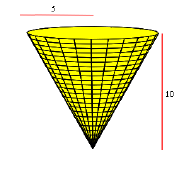
\includegraphics[]{cono.PNG}
\end{center}
Los datos que tenemos son los siguientes:\\
En primer lugar, sabemos que el agua varía 9 $m^3/min$, es decir $\dfrac{dV}{dt} = 9$\\
Lo que debemos determinar es $\dfrac{dh}{dt}$ cuando $h=6$\\
\\
Recordemos que el volumen de un cono se define como
$$V = \dfrac{\pi r^2 h}{3}$$
Además, sabemos por las dimensiones del cono, que
$$\dfrac{r}{h} = \dfrac{5}{10}$$
Por lo que 
$$r = \dfrac{h}{2}$$
Luego,
$$V = \dfrac{\pi h^3}{12}$$
Derivando esto implícitamente en función de $t$ (notar que ambas variables habrá que derivarlas en otra variable), tenemos
$$\dfrac{dV}{dt} = \dfrac{\pi}{12}3h^2\dfrac{dh}{dt}$$
Despejando $\dfrac{dh}{dt}$,
$$\dfrac{dh}{dt} = \dfrac{4}{\pi h^2} \cdot \dfrac{dV}{dt}$$
Finalmente, reemplazamos con $\dfrac{dV}{dt} = 9$ y $h = 6$, obteniendo
$$\dfrac{dh}{dt} = \dfrac{4}{36\pi}\cdot 9 = \dfrac{1}{\pi} m/min$$
\end{solucion}
\item La ley de los gases para un gas ideal a la temperatura absoluta $T$ (en Kelvin) y la presión $P$ (en atmósferas) con un volumen $V$ (en litros) es
$$PV = nRT$$
donde $n$ es constante y corresponde al número de moles del gas y $R = 0,0821$ es la constante de los gases.\\
Suponga que en el instante $t_0$ la presión $P$ es igual a 8 $atm$ y que esta aumenta a razón de 0,1 $atm/min$. Además se sabe que en ese mismo instante el volumen $V$ es de 10 litros y que este disminuye a razón de 0,15 $lt/min$.\\
Determine la razón de cambio de $T$, con respecto al tiempoo, en el instante $t_0$, sabiendo que la constante $n = 10\ mol$.
\begin{solucion}
En el instante $t_0$, tenemos
$$P = 8\ atm, \qquad P' = 0.1\ atm/min$$
$$V = 10\ l, \qquad V' = -0.15\ l/min$$
Además, estamos buscando
$$T'(t=t_0)$$
Olvidemos esto por ahora y veamos como se relacionan las variables en cualquier instante $t$.\\

En cualquier instante $t$, se cumple que
$$PV = 10 \cdot 0.0821 \cdot T \ra PV = 0.821 T $$
Derivando esto en función del tiempo (de manera implícita para todas las variables), tenemos
$$P'V + V'P = 0.821T'$$
Despejamos $T'$, ya que es lo que queremos obtener,
$$T' = \dfrac{P'V + V'P}{0.821}$$
Finalmente, evaluamos en $t_0$, es decir, reemplazamos los datos entregados en el enunciado, esto es
$$T'(t=t_0) = \dfrac{8 \cdot (-0.15) + 10 \cdot 0.1)}{0.821} = -\dfrac{0.2}{0.821} = -0.243$$
Por lo que la razón de cambio de la temperatura es $-0.243\ K/min$
\end{solucion}
\item Para cada una de las siguientes funciones, encontrar sus máximos y mínimos locales, en caso de haber
\begin{tasks}(2)
\task $f(x) = x^4 - 8x^2 + 3$
\task $f(x)=x+ln(x^2-1)$
\end{tasks}
\begin{solucion}

\begin{enumerate}[a)]
\item $f(x) = x^4 - 8x^2 + 3$\\
\\
En primer lugar, buscamos los puntos críticos, esto es
$$f'(x) = 4x^3 - 16x = 0$$
$$4x(x^2 - 4) = 0$$
$$4x(x+2)(x-2) = 0$$
$$x = -2, \qquad x = 0, \qquad x = 2$$
Luego, obtenemos la segunda derivada,
$$f''(x) = 12x^2 - 16$$
Y evaluamos en los puntos críticos para clasificarlos
$$f''(-2) = 48 - 16 > 0 \ra \text{mínimo local}$$
$$f''(0) = -16 < 0 \ra \text{máximo local}$$
$$f''(2) = 48 - 16 > 0 \ra \text{mínimo local}$$
Finalmente, evaluamos estos puntos en la función original para obtener los máximos y mínimos locales
$$f(-2) = -13 \ra \text{mínimo local}$$
$$f(0) = 3 \ra \text{máximo local}$$
$$f(2) = -13 \ra \text{mínimo local}$$
\item $f(x)=x+ln(x^2-1)$\\
\\
En primer lugar, notemos que el dominio de $f$ corresponde a 
$$x^2-1 > 0 \ra x \in (-\infty, -1) \cup (1, \infty)$$
Luego, derivamos para encontrar los puntos críticos,
$$f'(x) = 1 + \dfrac{2x}{x^2-1} = \dfrac{x^2 +2x -1}{x^2-1} = 0$$
Utilizando la formula de la ecuación de segundo grado,
$$x = -1 + \sqrt[]{2}, \qquad x = -1 - \sqrt[]{2}$$
Sin embargo, notemos que $-1 < -1 + \sqrt[]{2} < 1$, por lo que no es un punto crítico, dado que no esta en el dominio de la función.

Ahora, derivamos nuevamente para clasíficar nuestro punto crítico,
$$f''(x) = 
\dfrac{2(x^2-1) - 4x^2}{(x^2-1)^2} = 
\dfrac{-2 - 2x^2}{(x^2-1)^2} < 0$$
$f''(x)$ es negativa para todo $x$, por lo que $x = -1 - \sqrt[]{2}$ es un máximo local.
\end{enumerate}
\end{solucion}
\item Determine el máximo y mínimo absoluto de la función 
$$f(x) = 2\cos (x) + \sin (2x)$$
en el intervalo $[0, 2\pi]$.
\begin{solucion}
Derivando, tenemos que
$$f'(x) = -2 \sin(x) + 2 \cos(2x)$$
Igualamos esto a cero para obtener los puntos críticos, esto es
$$f'(x) = -2 \sin(x) + 2 \cos(2x) = 0 \ra \sin(x) = \cos(2x)$$
Para resolver esto, podemos hacerlo analíticamente graficando ambos lados de la igualdad, es decir,
\begin{center}
	\begin{tikzpicture}
	\begin{axis}[ 
	width=320pt,compat=1.5.1,grid style={ultra thin},every axis plot post/.append style={thick},
	x tick label style={font=\tiny},y tick label style={font=\tiny},
	scale only axis,grid=major,axis lines=middle,
	xlabel={$x$},
	ylabel={$y$},
	xmin=0,
	xmax=360,
	domain=-0:360,
	ymin=-1,
	ymax=1,
	xtick={0, 30, 90, 150, 180, 270, 360},
	xticklabels={$0$,$\dfrac{\pi}{6}$, $\dfrac{\pi}{2}$, $\dfrac{5\pi}{6}$,$\pi$,$\dfrac{3\pi}{2}$,$2\pi$},
	ytick={-1, 0, 1},
	legend style={at={(0.5,-0.05)},anchor=north,nodes={right}},
	] 
	\addplot[mark=none,color=blue, samples=500]{sin(x)}; 
	\addplot[mark=none,color=blue, samples=500]{cos(2*x)};
	\end{axis}
	\end{tikzpicture}
\end{center}
Aqui vemos claramente que hay 3 valores para los cuales las funciones se igualan. Probando para verificar, podemos concluir que estos son
$$x = \dfrac{\pi}{6}, \qquad x = \dfrac{5\pi}{6}, \qquad x = \dfrac{3\pi}{2}$$
Luego, nuestros candidatos a máximos y mínimos serán los puntos críticos y los bordes del intervalo, es decir
$$0, \quad \dfrac{\pi}{6}, \quad \dfrac{5\pi}{6}, \quad \dfrac{3\pi}{2}, \quad 2\pi$$
Evaluando, podemos ver que
$$f(0) = 2, \quad f(\dfrac{\pi}{6}) = \dfrac{3\ \sqrt[]{3}}{2}, \quad f(\dfrac{5\pi}{6}) = -\dfrac{3\ \sqrt[]{3}}{2}, \quad f(\dfrac{3\pi}{2}) = 0, \quad f(2\pi) = 2$$
Por lo que el mínimo es $-\dfrac{3\ \sqrt[]{3}}{2}$ y el máximo es $\dfrac{3\ \sqrt[]{3}}{2}$.
\end{solucion}
\item Encuentre los máximos y mínimos globales de la función
$$f(x) = \dfrac{|x|}{1+x^2}$$
en el intervalo $x \in [-3,2]$
\begin{solucion}
Notemos que podemos escribir $f(x)$ como
$$f(x)= \begin{cases}
\dfrac{x}{1+x^2} & x \geq 0\\\\
\dfrac{-x}{1+x^2} & x < 0
\end{cases}$$
Esta función no es derivable en $x=0$, sin embargo, podemos derivar a ambos lados y luego ver que ocurre. Entonces, derivando ambos lados por separado, tenemos que
$$x > 0 \ra f'(x) = \dfrac{(1+x^2) - 2x^2}{(1+x^2)^2} = \dfrac{1-x^2}{(1+x^2)^2} = \dfrac{(1+x)(1-x)}{(1+x^2)^2}$$
$$x < 0 \ra f'(x) = \dfrac{-(1+x^2) + 2x^2}{(1+x^2)^2} = \dfrac{x^2-1}{(1+x^2)^2} = \dfrac{(x+1)(x-1)}{(1+x^2)^2}$$
De aquí, obtenemos los puntos $x=1$ y $x=-1$ como puntos críticos. Además, debemos agregar a los puntos críticos, los bordes de nuestro intervalo y el punto donde la función no es derivable, es decir, $x=-3$, $x=2$ y $x=0$.\\

Ahora, evaluamos en cada uno de ellos, obteniendo
$$f(-3) = \dfrac{3}{10},\ f(-1) = \dfrac{1}{2}, \ f(0) = 0, \ f(1) = \dfrac{1}{2}, \ f(2) = \dfrac{2}{5}$$
Finalmente, el máximo es $\dfrac{1}{2}$ y el mínimo es $0$.
\end{solucion}
\item Estudiar, según el valor de la constante $k$, los puntos críticos y los puntos de inflexión de la función
$$f(x) = x^3-3kx^2+12x$$
\begin{solucion}
En primer lugar, calculemos las derivadas de $f$, esto es
$$f'(x) = 3x^2 - 6kx + 12$$
$$f''(x) = 6x - 6k$$
Para buscar los puntos críticos, igualamos la primera derivada a 0, con lo que
$$3x^2 - 6kx + 12 = 0 \ra x^2 - 2kx + 4= 0 \ra x = \dfrac{2k \pm \sqrt[]{4k^2-16}}{2} \ra x = k \pm \sqrt[]{k^2-4}$$
Con respecto a los puntos de inflexión, igualando la segunda derivada a 0 podemos ver que
$$6x- 6k = 0 \ra x = k,$$
por lo que siempre habrá un punto de inflexión en $x=k$\\

Luego, tendremos los siguientes escenarios.\\

Para $k \in (-2,2)$, no habrá ningún punto crítico, ya que la ecuación anterior no tiene solución.\\

Para $k = 2 y k = -2$, habrá un punto crítico en $x=k$. Además, este punto crítico será un punto de inflexión.\\

Para $k\in (-\infty, -2) \cup (2, \infty)$, habrán dos puntos críticos en 
$$x = k + \sqrt[]{k^2-4} \qquad y \qquad x = k - \sqrt[]{k^2-4}$$
Notemos además que para $x < k \ra f''(x) < 0$ y para $x > k \ra f''(x) > 0$, por lo que el punto crítico $x = k + \sqrt[]{k^2-4} > k$ corresponderá a un mínimo y $x = k - \sqrt[]{k^2-4} < k$ corresponderá a un máximo.
\end{solucion}
\item Probar que la ecuación $1+2x+3x^2+4x^3=0$ tiene solución única.
\begin{solucion}
Para demostrar esto debemos hacer dos cosas. En primer lugar, debemos demostrar que la ecuación tiene alguna solución (TVI) y en segundo lugar, debemos demostrar que esta no tiene más de una solución (TVM).\\

Para demostrar que la ecuación tiene alguna solución, definimos la función auxiliar
$$f(x) = 1+2x+3x^2+4x^3$$
Al evaluar, podemos ver que
$$f(0) = 1, \qquad f(-1) = -2$$
Notemos que $f$ es una función continua en todos los reales. Luego, por TVI, 
$$\exists c \in (-1,0) \text{ tal que } f(c) = 0$$
Para demostrar que la ecuación no tiene más de una solución, lo haremos por contradicción. Digamos que la ecuación tiene 2 soluciones, $x_1$ y $x_2$ con $x_1 < x_2$.\\

Luego, $f(x_1) = 0$ y $f(x_2) = 0$. Entonces, por TVM
$$\exists c \in (x_1, x_2) \text{ tal que } f'(c) = \dfrac{f(x_2) - f(x_1)}{x_2-x_1} = 0$$
Sin embargo, notemos que
$$f'(x) = 12x^2 + 6x + 2$$
Corresponde a una ecuación de segundo grado con determinante 
$$\Delta = 6^2-4\cdot 12 \cdot 2 = -60 < 0,$$
por lo que no tiene solución real. Esto es una contradicción con nuestra suposición anterior, por lo que la ecuación no puede tener dos soluciones.\\

En conclusión, la ecuación tiene solución única. 
$$\blacksquare$$
\end{solucion}
\item Demuestre que la ecuación $\sin (x) = 2x-1$ tiene exáctamente una raíz real.
\begin{solucion}
Para demostrar esto debemos hacer dos cosas. En primer lugar, debemos demostrar que la ecuación tiene alguna solución (TVI) y en segundo lugar, debemos demostrar que esta no tiene más de una solución (TVM).\\

Para demostrar que la ecuación tiene alguna solución, definimos la función auxiliar
$$f(x) = \sin x - 2x + 1$$
Al evaluar, podemos ver que
$$f(0) = 1, \qquad f(2) = \sin 2 - 3 < 0$$
Notemos que $f$ es una función continua en todos los reales. Luego, por TVI, 
$$\exists c \in (0,2) \text{ tal que } f(c) = 0$$
Para demostrar que la ecuación no tiene más de una solución, lo haremos por contradicción. Digamos que la ecuación tiene 2 soluciones, $x_1$ y $x_2$ con $x_1 < x_2$.\\

Luego, $f(x_1) = 0$ y $f(x_2) = 0$. Notemos que $f$ es derivable en todos los reales. Entonces, por TVM
$$\exists c \in (x_1, x_2) \text{ tal que } f'(c) = \dfrac{f(x_2) - f(x_1)}{x_2-x_1} = 0$$
Sin embargo, notemos que
$$f'(x) = \cos x - 2 = 0 \ra \cos x = 2$$
Lo que no se cumple para ningún $x$, por lo que no existe ningún $c$ donde $f'(c) = 0$.\\

Esto es una contradicción con nuestra suposición anterior, por lo que la ecuación no puede tener dos soluciones.\\

En conclusión, la ecuación tiene solución única. 
$$\blacksquare$$
\end{solucion}
\item Sea $f$ una función derivable en $[0, \infty)$, tal que $\forall x \in [0, \infty)(f(2x)=2f(x))$.\\
Demuestre que
$$\forall x \in (0, \infty) \exists c > 0 \left(f'(c) = \dfrac{f(x)}{x}\right)$$
\begin{solucion}
La función $f$ es derivable en el intervalo $[x, 2x]$ para $x \geq 0$. Luego, por TVM,
$$\exists c \in (x,2x) \text{ tal que } f'(c) = \dfrac{f(2x)-f(x)}{2x-x} = \dfrac{2f(x)-f(x)}{x} = \dfrac{f(x)}{x}$$
Por lo tanto,
$$\forall x \in (0, \infty) \exists c > 0 \left(f'(c) = \dfrac{f(x)}{x}\right)$$
\end{solucion}
\item Si $f$ es una función dos veces derivable en $[a,b]$ tal que $f(a)=f(b)=0$ y $f(c) > 0$ con $a < c < b$, demuestre que
$$\exists \alpha \in (a,b) (f''(\alpha) < 0)$$
\begin{solucion}
Como $f$ es dos veces derivable en $[a,b]$ y $a < c < b$, entonces $f$ cumple con las condiciones del TVM en los intervalos $[a,c]$ y $[c,b]$, Aplicando TVM en ambos, tenemos que
$$\exists \alpha_1 \in (a,c) \text{ tal que } f'(\alpha_1) = \dfrac{f(c)-f(a)}{c-a} = \dfrac{f(c)}{c-a} > 0$$
$$\exists \alpha_2 \in (c,b) \text{ tal que } f'(\alpha_2) = \dfrac{f(b)-f(c)}{b-c} = -\dfrac{f(c)}{b-c} < 0$$
Notemos ahora que 
$$a < \alpha_1 < c < \alpha_2 < b$$
Además, como $f''$ es derivable en $[a, b]$, las condiciones del TVM también se cumplen para $f''$ en el intervalo $[\alpha_1, \alpha_2]$. Luego, por TVM,
$$\exists \alpha \in (\alpha_1, \alpha_2) \text{ tal que } f''(\alpha) = \dfrac{f'(\alpha_2) - f'(\alpha_1)}{\alpha_2 - \alpha_1} < 0$$
Esto último lo sabemos por los signos de $f'(\alpha_1)$ y $f'(\alpha_2)$ que fueron concluidos anteriormente.
$$\blacksquare$$
\end{solucion}
\item Determine los siguientes límites, en caso de que existan
\begin{tasks}(3)
\task $\lim\limits_{x\ra 0}\dfrac{(\arcsin x)^2}{1-cos(3x)}$
\task $\lim\limits_{x\ra 0} x^{\frac{1}{\ln (e^x-1)}}$
\task $\lim\limits_{x\ra \infty} \left(1+\dfrac{a}{x}\right)^{bx}$
\end{tasks}
\begin{solucion}

\begin{enumerate}[a)]
\item $\lim\limits_{x\ra 0}\dfrac{(\arcsin x)^2}{1-cos(3x)}$\\
\\
Notemos que al evaluar, este límite es de la forma $\dfrac{0}{0}$, por lo que podemos aplicar L'Hopital, esto es
{\footnotesize$$\lim\limits_{x\ra 0}\dfrac{(\arcsin x)^2}{1-cos(3x)} 
\stackrel{L'H}{=} \lim\limits_{x\ra 0}\dfrac{((\arcsin x)^2)'}{(1-cos(3x))'} 
= \lim\limits_{x\ra 0}\dfrac{2(\arcsin x)\dfrac{1}{\sqrt[]{1-x^2}}}{3\sin(3x)}
= \lim\limits_{x\ra 0}\dfrac{2(\arcsin x)}{3\ \sqrt[]{1-x^2}\sin(3x)} $$}\\
Notemos que al evaluar este último, seguimos obteniendo $\dfrac{0}{0}$, por lo que debemos aplicar L'Hopital nuevamente,
{\scriptsize$$\lim\limits_{x\ra 0}\dfrac{2(\arcsin x)}{3\ \sqrt[]{1-x^2}\sin(3x)}
\stackrel{L'H}{=} \lim\limits_{x\ra 0}\dfrac{(2(\arcsin x))'}{(3\ \sqrt[]{1-x^2}\sin(3x))'}
=\lim\limits_{x\ra 0}\dfrac{\dfrac{2}{\sqrt[]{1-x^2}}}{3\dfrac{1}{2\ \sqrt[]{1-x^2}}\cdot(-2x)\sin(3x) + 3\ \sqrt[]{1-x^2}\cos(3x)3} $$}\\
Evaluando esto, tenemos que
$$\lim\limits_{x\ra 0}\dfrac{(\arcsin x)^2}{1-cos(3x)} = \dfrac{2}{9}$$
\item $\lim\limits_{x\ra 0} x^{\frac{1}{\ln (e^x-1)}}$\\
\\
En primer lugar, notemos que
$$\lim\limits_{x\ra 0} x^{\frac{1}{\ln (e^x-1)}} = 
\lim\limits_{x\ra 0} e^{\ln(x^{\frac{1}{\ln (e^x-1)}})} = 
\lim\limits_{x\ra 0} e^{\frac{ln(x)}{\ln (e^x-1)}} = 
e^{\lim\limits_{x\ra 0}\frac{ln(x)}{\ln (e^x-1)}}$$
Por lo tanto, lo que haremos será resolver el límite del exponente y luego elevar $e$ con el resultado obtenido para finalmente obtener el límite pedido.\\

Es decir, debemos resolver
$$\lim\limits_{x\ra 0}\frac{ln(x)}{\ln (e^x-1)}$$
Notemos que al evaluar, obtenemos $\dfrac{\infty}{\infty}$, por lo que podemos aplicar L'Hopital, esto es
$$\lim\limits_{x\ra 0}\frac{ln(x)}{\ln (e^x-1)} \stackrel{L'H}{=}
\lim\limits_{x\ra 0}\frac{\dfrac{1}{x}}{\dfrac{e^x}{e^x-1}} =
\lim\limits_{x\ra 0}\frac{e^x-1}{xe^x}  \stackrel{L'H}{=} 
\lim\limits_{x\ra 0}\frac{e^x}{e^x + xe^x} = 1$$
No olvidemos que esto corresponde al exponente del límite pedido, por lo que 
$$\lim\limits_{x\ra 0} x^{\frac{1}{\ln (e^x-1)}} = e^1 = e$$
\item $\lim\limits_{x\ra \infty} \left(1+\dfrac{a}{x}\right)^{bx}$\\
\\
De forma similar, al ejercicio anterior, tenemos que
$$\lim\limits_{x\ra \infty} \left(1+\dfrac{a}{x}\right)^{bx} =
\lim\limits_{x\ra \infty} e^{\ln\left(\left(1+\frac{a}{x}\right)^{bx}\right)} =
\lim\limits_{x\ra \infty} e^{bx\ln\left(1+\frac{a}{x}\right)} =
e^{\lim\limits_{x\ra \infty} bx\ln\left(1+\frac{a}{x}\right)}$$
Luego, debemos resolver
$$\lim\limits_{x\ra \infty} bx\ln\left(1+\dfrac{a}{x}\right)$$
Notemos que este límite es de la forma $\infty \cdot 0$.\\

Reordenando,
$$\lim\limits_{x\ra \infty} bx\ln\left(1+\dfrac{a}{x}\right) =
\lim\limits_{x\ra \infty} \dfrac{\ln\left(1+\dfrac{a}{x}\right)}{\dfrac{1}{bx}} = \dfrac{0}{0} $$
Luego,
{\scriptsize$$\stackrel{L'H}{=} \lim\limits_{x\ra \infty}  \dfrac{\dfrac{-\frac{a}{x^2}}{1+\frac{a}{x}}}{-\dfrac{b}{(bx)^2}} =
\lim\limits_{x\ra \infty} \dfrac{\dfrac{\frac{a}{x^2}}{\frac{a+x}{x}}}{\dfrac{1}{bx^2}} =
\lim\limits_{x\ra \infty} \dfrac{\dfrac{ax}{x^2(a+x)}}{\dfrac{1}{bx^2}} =
\lim\limits_{x\ra \infty} \dfrac{abx^3}{x^2(a+x)} =
\lim\limits_{x\ra \infty} \dfrac{abx}{a+x} \stackrel{L'H}{=} 
\lim\limits_{x\ra \infty} ab = ab$$}\\
Finalmente,
$$\lim\limits_{x\ra \infty} \left(1+\dfrac{a}{x}\right)^{bx} = e^{ab}$$
\end{enumerate}
\end{solucion}
\item Determine las asíntotas de la función $f(x) = xe^{1/x}$.
\begin{solucion}
En primer lugar, veamos las asíntotas verticales. Notemos que la función solo se indefine en $x=0$, por lo que este es el único candidato a asíntota vertical.\\

Verificamos,
$$\lim\limits_{x \ra 0} xe^{1/x} = 
\lim\limits_{x \ra 0} \dfrac{e^{1/x}}{\dfrac{1}{x}} \lh
\lim\limits_{x \ra 0} \dfrac{-\dfrac{e^{1/x}}{x^2}}{-\dfrac{1}{x^2}} =
\lim\limits_{x \ra 0} e^{1/x} =
e^{\infty} = \infty
$$
Por lo tanto, $x = 0$ es una asíntota vertical.\\

Para ver las asíntotas horizontales, hacemos
$$\lim\limits_{x \ra \pm \infty} xe^{1/x} = \pm \infty e^0 = \pm \infty$$
Por lo que no hay asíntotas horizontales.\\

Por último, buscamos asíntotas oblicuas con
$$m = 
\lim\limits_{x \ra \pm \infty} \dfrac{f(x)}{x} =
\lim\limits_{x \ra \pm \infty} \dfrac{xe^{1/x}}{x} =
\lim\limits_{x \ra \pm \infty} e^{1/x} =
1$$
$$n = 
\lim\limits_{x \ra \pm \infty} f(x) - mx =
\lim\limits_{x \ra \pm \infty} xe^{1/x} - x =
\lim\limits_{x \ra \pm \infty} x(e^{1/x} - 1) =
\lim\limits_{x \ra \pm \infty} \dfrac{e^{1/x} - 1}{\dfrac{1}{x}}$$
$$\lh
\lim\limits_{x \ra \pm \infty} \dfrac{-\dfrac{e^{1/x}}{x^2}}{-\dfrac{1}{x^2}} =
\lim\limits_{x \ra \pm \infty} e^{1/x} = 1
$$
Por lo que $y = x + 1$ es asíntota oblicua.
\end{solucion}
\end{preguntas}
\end{document}